\documentclass{beamer}
\usepackage{beamerthemeboxes}
\usepackage[utf8]{inputenc}
\usepackage{times}
\usepackage{palatino, url, multicol}

\mode<presentation>
{
  \usetheme{Warsaw}
  %\usetheme{Ilmenau}
  % or ...

  % or whatever (possibly just delete it)
   \usefonttheme[onlylarge]{structuresmallcapsserif}

    \usecolortheme{beetle}

    \setbeamerfont{title}{shape=\itshape,family=\rmfamily}

}


\providecommand{\e}[1]{\ensuremath{\times 10^{#1}}}

\title[Strumenti Didattici per Embedded]{Sviluppo di Strumenti Didattici
per la Programmazione Embedded}
\author{Michele Bianchi}
\usepackage{graphicx}
\date{22 Settembre 2010}
\begin{document}
   \section{Introduzione}
	\frame{
		\titlepage
	}
   \subsection{Struttura}
	\frame{
		\frametitle{Introduzione}
 		\begin{block}{Difficoltà nella programmazione Embedded}
            \begin{itemize}
                \item Linguaggi di basso livello
                \item Difficoltà nel debugging
            \end{itemize}
        \end{block}
	    \begin{block}{Soluzione proposta}
            Collegamento tra il pacchetto di modellazione di sistemi
            discreti SciCos e il sistema embedded NXT 
        \end{block}
    }
   
   \subsection{NXT/SPAM}
   \frame{
        \frametitle{LEGO MINDSTORM NXT e SPAM}

            \begin{columns}
                \column{.40\textwidth}
                    \textbf{LEGO MINDSTORM NXT}

                    ~~~Piattaforma Embedded per la creazione di robot e
                    sistemi automatici.

                    \hspace{1\textheight}
                    \textbf{Caratteristiche}

                    \begin{itemize}
                    \item Piattaforma ATMEL AT91SAM7
                    \item Controller Bluetooth
                    \item Connessione USB
                    \item Bus I$^2$C
                    \end{itemize}

                \column{.05\textwidth}
                \column{.55\textwidth}
                    \begin{figure}[h]
                    \centering
                    \includegraphics[scale=0.05]{../Pictures/SPAM.jpg}
                    \end{figure}

                    \begin{block}{SPAM}
                        \begin{itemize}
                         \item Due motori indipendenti
                         \item Sensore di luce
                         \item Sensore brandeggiabile di distanza 
                        \end{itemize}
                    \end{block}
            \end{columns}

   }


   \subsection{nxtOSEK}
	\frame{
		\frametitle{nxtOSEK}
        Sistema operativo per LEGO NXT
        \begin{block}{Features}
            \begin{itemize}
                \item Scritto in C
                \item Primitive OSEK/ATK e $\mu$Itron
                \item Device Drivers LeJOS NXJ
            \end{itemize}
        \end{block}
        \begin{block}{Alternative}
            \begin{itemize}
                \item nxOS
                \item NXC/NBC
            \end{itemize}
        \end{block}

    }

   \subsection{PID Controller}
    \frame{
        \frametitle{Digital PID Controller}
        \begin{block}{Caratteristiche}
           \begin{itemize}
            \item Sistema di controllo ciclico
            \item Cerca di minimizzare l'errore da iterazione ad iterazione
           \end{itemize}
        \end{block}

        \begin{block}{PID su SPAM}
            \begin{itemize}
             \item Utilizzato per il controllo dei Servo Motori
             \item Raggiunge la velocità richiesta dopo un breve periodo di
                oscillazione
             \item Più alta è la velocità obiettivo più lungo è il periodo
                di oscillazione
            \end{itemize}
        \end{block}
    }
   \section{Progetto}
    
    \frame{
        \title{Overview del progetto}

        \begin{itemize}
            \item Client eseguito su SPAM
            \item Applicazione Server che comunica col Client e con SciCos
            \item Blocchi d'interfaccia per SciCos
        \end{itemize}

        \begin{figure}[h]
            \centering
            \includegraphics[width=.8\textwidth]{../Images/BROFistInteractions.png}
        \end{figure}
    }

   \subsection{Client}
	\frame{
		\frametitle{Client}		
		\begin{itemize}
		    \item Riceve i comandi dal server
            \item Risponde a richieste sui sensori
            \item Contiene un PID Controller
            \item Stampa qualche dato a video
       \end{itemize}
       
       \begin{block}{Comunicazione col PC}
        \begin{itemize}
            \item Comunicazione USB tra nxtOSEK e PC problematica
            \item Scelta ricaduta sul Bluetooth
            \item Latenza alta $\sim{}45ms$
        \end{itemize}
       \end{block}
       
    }
  
  \subsection{Server}
	\frame{
		\frametitle{Server}
		\begin{itemize}
         \item Si connette a SPAM via Bluetooth
         \item Attende connessioni da parte di SciCos via IPC Socket
         \item Fa da bridge tra SciCos e SPAM
	  	\end{itemize}
        Permette estensioni di facile sviluppo.
	}
  \subsection{SciCos}
	\frame{
		\frametitle{SciCos}
        SciCos è il pacchetto di modellazione grafica di sistemi discreti
        di SciCosLab.
        \begin{columns}
        \column{.45\textwidth}
        \begin{figure}[h]
            \centering
            \includegraphics[scale=.25]{../Images/Yadda.png}
        \end{figure}
        \column{.05\textwidth}
        \column{.5\textwidth}
        \begin{itemize}
            \item Alternativa Open Source a Matlab
            \item Estensibile tramite la scrittura di funzioni in C
            \item Multipiattaforma
        \end{itemize}

        \end{columns}
	}
   \subsection{Blocchi BROFist}
	\frame{
		\frametitle{Blocchi d'interfaccia per SciCos}
        \begin{figure}[h]
            \centering
            \includegraphics[width=1\textwidth]{../Images/SciCosScreen.png}
        \end{figure}

%        \begin{columns}
%            \column{.425\textwidth}
%              \begin{itemize}
%                \item BRO\_Controller
%                \item SENS\_Disp
%                \item MOTOR\_Disp
%              \end{itemize}
%            \column{.05\textwidth}
%            \column{.425\textwidth}
%              \begin{itemize}
%                \item SPAM\_Sensor
%                \item SPAM\_Motor
%              \end{itemize}
%        \end{columns}
	}
   \section{Conclusioni}
   \subsection{Sviluppi Futuri}
	\frame{
		\frametitle{Sviluppi Futuri}
		\begin{columns}
            \column{.55\textwidth}
            \begin{figure}[h]
                \centering
                \includegraphics[width=1\textwidth]{../Images/TheBROFistStructureSlides.png}
            \end{figure}

            \column{.05\textwidth}
            \column{.4\textwidth}
              \begin{itemize}
                \item Aggiunta del supporto USB
                \item Creazione di applicazioni in locale che sfruttano il
                    Server
                \item Creazione di applicazioni remote come un sito web
                    che, attraverso il server, controlla un NXT da remoto
              \end{itemize}
        \end{columns}
	}

    \subsection{Conclusioni}
     \frame{
        \frametitle{Contributo della tesi}
        \begin{itemize}
            \item Client per NXT che comunica col PC,
                permettendo il controllo remoto, anche attraverso PID
                Controller
            \item Server che comunica tra NXT e PC, il quale può venir
                esteso per permettere nuove connessioni
            \item Blocchi di Interfaccia per SciCos per modellare dei
                sistemi discreti per NXT con un feedback reale
        \end{itemize}
     }


   \frame{
       \begin{center}
            \Huge{Domande?}
       \end{center}
   }
\end{document}
